\documentclass[12pt, a4paper]{article}

\usepackage{listings}
\usepackage{color}
\usepackage{enumitem}
\usepackage{amsthm}
\usepackage{amssymb}
\usepackage{listings}
\usepackage{setspace}
\usepackage{graphicx}
\graphicspath{ {./figures/} }


\title{Introduction to Neurobiology}
\author{William Darko}
\date{Summer 2021}

\pagenumbering{arabic}

\begin{document}

\maketitle
\newpage

\tableofcontents

\newpage

\section{About this course}
\paragraph*{}
Objective of the course is to learn how the nervous system produces behaviour,
how we use our brains in our day to day lives, and how neuroscience can help explain
the problems afflicting people today. There'll be focus on functional human neuroanatomy,
and neuronal communication, to help understand how we perceive the world, do body movements,
and interact with others.

\newpage

\section{Resources}

\begin{itemize}
    \item \textbf{Coursera: Understanding the Brain: The Neurobiology of Everyday Life}
    taught by professor of Neurobiology Peggy Mason, at the University of Chicago (https://www.coursera.org/learn/neurobiology)
\end{itemize}

\newpage

\section{Introduction}
\begin{itemize}
    \item \textbf{The Diving Bell and the Butterfly}: 
    Jean-Dominique Bauby, locked-in syndorme.
\end{itemize}

\section{The Nervous System}
\subsection{The Four Functions}
The locked-in syndrome tells of the four basic functions of the brain/central nervous system.
\begin{enumerate}
    \item \textbf{Voluntary Movement:} Every thing we do that is driven by the brain,
    both deliberate actions, such jumping, speaking, raising your hand, etc, and not so deliberate
    actions like wincing in reaction to stepping on a lego piece.
    \item \textbf{Perception:} Perception is distinct from sensation; its what we conciously
    appreciate about sensation. Its what we're capable of being aware of such as vision, hearing,
    smell, taste, balance, position, lung pressure, etc.
    \item \textbf{Homeostasis:} Used to keep body within its physiological limits.
    For example, making sure the body has enough oxygen, the right blood pressure, right body temperature.
    Also, homeostasis accounts for life cycle events like a mother giving birth, and the conditions 
    needed for the child to be healthy. Altogether, a process of maintaining healthy internal conditions.
    \item \textbf{Abstract functions:} Higher functions of the central nervous system like
    thinking, language, motivation, feeling emotion, etc. Also, plays a huge role in how we interact with other humans.
\end{enumerate}

\subsection{Central Anatomy}
Mapping of the four functions to regions of the brain.
\begin{enumerate}
    \item Motor neurons which exist in the brain stem, or the spinal cord are responsible
    for \textbf{voluntary movement}. There are less than 100,000 motor neurons, out of about 200 billion
    in the entire nervous system. Motor neurons in the brain system are responsible of movement of the mouth, face,
    hence speech, facial expressions, swallowing, etc.
    Motor neurons in the spinal cord are responsible for bodily movements like movement of the arms,
    legs, etc.
    \item \textbf{Perception} is entirely in the \textbf{Forebrain}; more specifically,  it depends entirely on the \textbf{Cerebral Cortex}.
    Perception is one of the higher brain functions; if the information carried by neurons does not 
    make it to to the Cerebral Cortex, then there's no perception; there's no concious appreciation/awareness
    of sensation.
    \item \textbf{Homeostasis} depends on the \textbf{Forebrain, brain stem, and spinal cord}.
    The forbrain's contribution to homeostasis is hormonal. The brain stem has a varied contribution; its responsible for
    the automatic changes we're not able to control, the autonomic (involuntary) functions of our nervous system. The spinal cord's
    contribution is similar to that of the brain stem.
    
    The brain stem, and spinal cord serve as pathways for information, both incoming, and outgoing. 

    \item \textbf{Abstract functions} are entirely in the forebrain, and function independent of the brain stem, and spinal cord.
    The forebrain is the "seat of conciousness"; all perception, and abstract conginitve functions like memory, depend on the forebrain;
    more specifically,the cerebral cortex.
\end{enumerate}

{
    \centering
    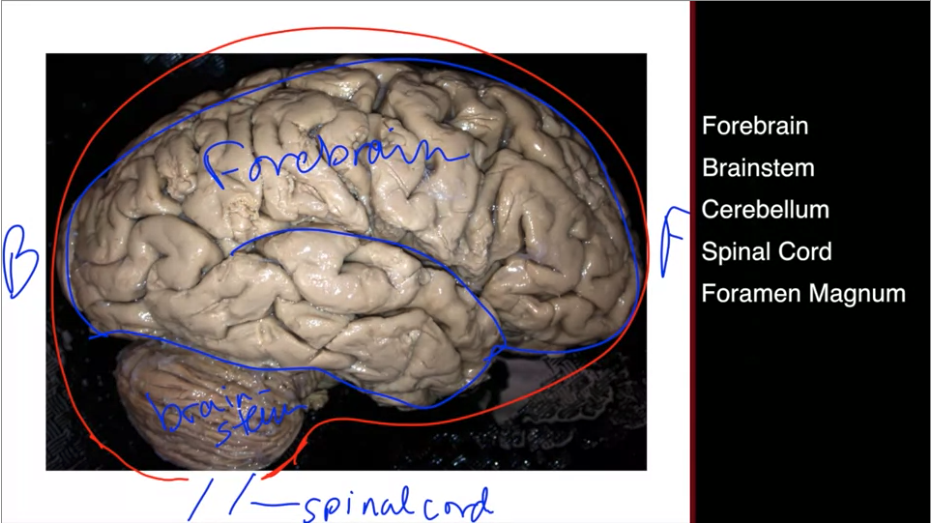
\includegraphics[width=8cm]{BrainImg_FromSide_SidesAnnotated.png}
    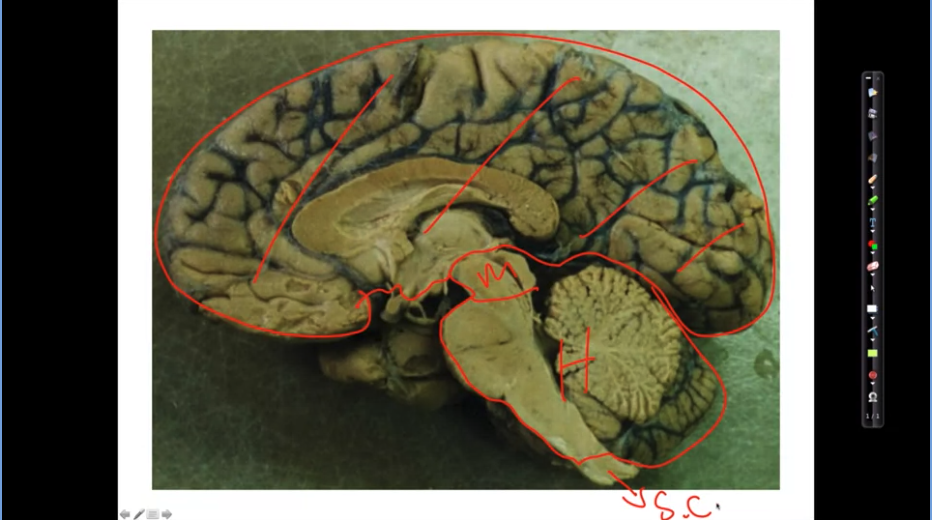
\includegraphics[width=8cm]{BrainImg_CutFromSide_MidHindBrainStem.png}

}
\newpage

\section{Neurons; the ``stars" of the nervous system"}

\subsection{Parts of the Neuron}
\paragraph*{}
There are four parts to neurons.
\begin{enumerate}
    \item Cell body, also known as the \textbf{Soma}. Place that keeps the cell going,
    makes all the materials needed for the entire neuron
    \item \textbf{Dendrites}; they branch out of the cell body, creating a \textbf{tree like structure
    called the dendritic arbour/tree}. They're responsible for gathering information for the neuron. Information 
    goes into the dendrites. Dendrites may be perceived as the ears of the neuron.
    \item Infomation processed locally from dendrites, sent out through one \textbf{axon} which is more gloablly distributed
    compared to the dendrites. Axon can travel a metre; and ultimately carry information to a \textbf{synaptic terminal}.
    \item \textbf{Synaptic terminals} are the point of information transfer between cells; infromation is carried to the terminal
    via axons. There's a small space between the synaptic terminal, and the receiving cell/dendrite; that space is where the
    event of information transfer occurs, which we know as a \textbf{synapse}.
\end{enumerate}

\subsection{Neuronal Uniqueness}
\paragraph*{}
A wide variety of ways the anatomy of neurons can make them different from each other.
Neurons also differ in the sense of what the neurons are connected to, what neurons are talking to; the inputs
and outputs. In addition to the \textbf{anatomy}, other differences include:
\begin{itemize}
    \item \textbf{Excitability}: how talkative is the neuron. How much work is needed
    to get neuron to fire action potentials. How likely or unlikely is it to fire action potentials.
    \item \textbf{Neurotransmitters}: What chemical/substance does the neuron use to communicate.
    For instance, some neurons use serotonin. How does the neuron ``speak''. Difference in communication speed.
    Affirmative vs negative.
\end{itemize}

\subsection{Glial cells}
\paragraph*{}
Neuron don't exist on their own, they requrie the support of Glial Cells. There's a one-to-one
mapping of neurons to glia. There's different types of Glial Cells:
\begin{enumerate}
    \item \textbf{Astrocytes}: behave as sanitation workers of the brain. They collect the refuse of neurons, such as excess ions, and 
    neurotransmitters. They also allow neurons to get to where they have to go during development. Synapses are envoloped in the processes of 
    Astrocytes, which helps with maintaining them. Comprice about 20 percent of glial cells
    \item \textbf{Oligodendrocytes (Central nervous sys.), and Schwann cells (Peripheral nervous sys.)}: Create
    myelin in their respective areas of the nervous system. Combined, these comprice about 75 percent of glial cells.
    \item \textbf{Microglia}: comprice about 5 percent of glia. Immune cells from the blood lineage that have invaded into the central nervous system,
    and are idle as long as the human body is health. However they react to areas of damage, and sometimes even contribute to the damage. Implicated in several diseases like
    chronic pain, and neurodegenerative disorders like alzheimer's.
\end{enumerate}

\subsection{Myelin}
\paragraph*{}
Meylin is a \textbf{fatty wrap that goes around some axons.} The difference between a myelinated axon, and an
unmeylinated axon/naked axon.
\begin{itemize}
    \item \textbf{Unmyelinated} axons can only transfer information at a slow rate; about
    \textbf{0.2 - 1.0 m/s}
    \item \textbf{Myelinated} axons have myelin applied and carry infromation orders of magnitude faster than naked axons.
    the speed at which these axons carry information increases to \textbf{2 - 120 m/s}. A speed inperceptible to us humans.
\end{itemize}
Myelinated axons are significant especially in cases where we need infromation fast such as infromation about our balance, which we need the fastest. Neurons
that support a posture against gravity, use myelinated axons.

The infomation that gets transferred through myelinated axons can be perceived as binary digits
\textbf{(011001110111...)}. Whats important about this sequence of binary digits is less about whether its a 1 0r 0, but 
more of the \textbf{pattern of 1's} that appear in the sequence. That is the neural code; the \textbf{1s represent
action potentials or spikes}. The \textbf{timing} of the spikes is what carries information.

The spikes that traverse through the myelinated axon travel so fast because they jump between the gaps of
the myelin wraps, thus not having to traverse through the wraps, and hence the entire physical
distance of the axon; effectively shortening the distance, and time required for the action potential to travel.
\\

{
    \centering
    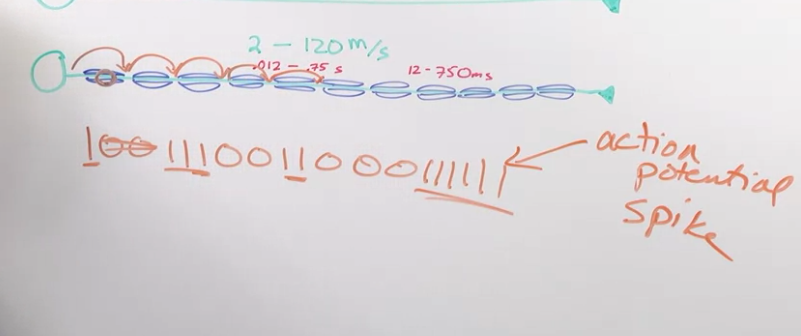
\includegraphics[width=10cm]{myelinated_axon_whiteboard.png}

    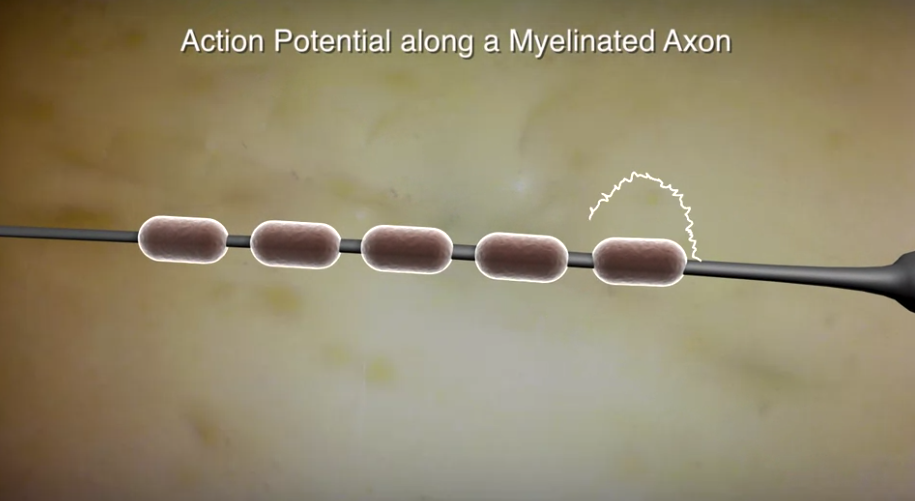
\includegraphics[width=10cm]{action_potential_myelinated_axon_animated.png}
    
}

\paragraph*{}
However, consider if along the myelinated axon, there becomes less, and less myelin wraps.
Our initial action potential, if starting as a string of bits say \textbf{001100111010110111101}, may come out on the other end
due to the decrease in myelin wraps as a completely incoherent message inconsistent with the initial one, say: \textbf{000001001000100000100}.
This is caused by what are known as \textbf{demyelinating diseases} which degrade the information transfer.

\subsection{Demyelinating Diseases}
\paragraph*{}
Recall that Glial Cells that create Myelin are either in central nervous system, or Peripheral nervous system. Thus people
who get demyelinating diseases either get it in the CNS, or PNS, but not both.

So the problem is either in the interaction between the \textbf{Oligodendrocytes} and the axon,
in which case we get a \textbf{Central Demyelinating Disease}, which the most common by far is \textbf{Multiple Sclerosis}.

Or, there's a problem in the Schwann cells, and its interaction between with the axons. In which case,
we get something like \textbf{Charcot-Marie-Tooth} which are a diverse group of heriditary demyelinating neuropathies.

Neural code is disrupted any where there is demyleination. Demyleination would mostly affect
motor axons which travel information the fastest. \textbf{Symptoms someone gets from Multiple Sclerosis would
depend on which axon group is affected}.

\section{Central Nervous System vs. Peripheral Nervous System}
Barrier between CNS, and PNS are made of three membranes; the meninges. There are 
\textbf{three meningeal layers that go from very weak, very tender (the pia) to very
tough (the dura)}

\subsection{Meninges}
\begin{itemize}
    \item Three meningeal layers
    \item \textbf{Pia} (very weak, most tender, and the inner most membrane; closer to the brain and spinal cord),
    \textbf{Arachnoid} (mid membrane, with spidery like structure). The \textbf{Dura} (outer most membrane, and the toughest)
    \item \textbf{Dura}, is the toughest sack, and what prevents concussions from happening all the time. It "floats"
    the brain in fluid and prevents it from banging about, and getting bruised.
    \item Neurons of these three membranes are entirely contained in the Central Nervous System
    \item The only neurons that leave the CNS are those that serve a motor function; these neurons
    \textbf{go out the meninges and into the periphery (PNS)}
    \item \textbf{Motor, and Autonomic neurons} that carry information from the CNS through the meninges, into the PNS
    \item \textbf{Sensory neurons} that carry information from the PNS, through the meninges to the CNS
    \item Neurons are either sensorial, or peripheral, based on where the cell body is, not where its
    axons, or dendrites are.
    \item Peripheral Neurons include \textbf{sensory, and autonomic} neurons, located in the autonomic ganglia
    \item These autonomic ganglia neurons, \textbf{share vulnerabilites with each other, but none with the neurons in the CNS}. A 
    consequence of this is diseases like Congenital Insensitivity to Pain; where people who suffer a genetic mutation
    that prevent a group of sensory neurons from developing, like those that respond to injury
    (they don't feel pain). 
\end{itemize}

\subsection{Peripheral Diseases}

\paragraph*{}
Diseases that affect that affect nervous system, affect either CNS, or PNS.
Meninges perfrom as a very effective barrier, that protects the CNS, from the diseases
that the PNS is often more vulnerable to than CNS. As a result, two regions (PNS, and CNS),
have different capacities for repair; PNS is better capable of repairing damage, as compared to the CNS.

Peripheral Nervous System is vulnerable to large molecules like \textbf{botulinum toxin}, viruses like \textbf{Polio},
\textbf{Herpes Zoster}.

\begin{itemize}
    \item \textbf{Botulinum Toxin}: comes from spoiled food, primarily affects
    peripheral nervous system. Doesn't get past meninges.
    \item \textbf{Polio}: unlike the botulinum toxin, \textbf{gets past the meninges}.
    Gets through to the meninges, by \textbf{entering between the synapse between the motor
    neuron and the voluntary muscle}, travelling through the the meninges by riding along
    the axon of a motor neuron. Once it gets through the meningeal layer, it \textbf{kills the motor neuron on 
    that side.} As a result, there'll be an inability to control that muscle, or conduct volutary movement to that neuron's corresponding motor actions.
    \item \textbf{Herpes Zoster}: produces what's commonly known as shingles.
    Blossoms, and makes copies of itself, inside cells in the sensory territory, causing a virus in that area,
    producing a rash on the skin.
\end{itemize}

\subsection{Brain Tumors}

\paragraph*{}
To understand the origins of brain tumors, we must know the basics of cancer.
Cancer tumors are cells that divide uncontrollably without limitations; they become immortal.
Not only do they divide limitlessly, but also, the spread from one region of the body, to another,
becoming bigger and bigger, and starting new tumors elsewhere. Hence, one source
of brain tumors: \textbf{Metastasis}; tumors that start elsewhere like the lung, or colon,
asn spread to the brain.

\textbf{Metastasis} is a massive problem for brain. Brain tumors that expand 
uncontrollably, are constrained within the fixed, unexpanding, bony container that is the cranium.
As a result, the limitless growth of tumors in the brain only increase pressure on the brain, which is problematic.

Besides metastasis, what are other sources of tumors in the brain? Neurons, fortunately
do not divide; they are what's called \textbf{Post-mitotic} cells. Neurons don't divide,
don't regenerate, have not any descendants; once they're born, they live, then die. Hence,
this leaves the development of brain tumors to other to other cells in the brain; primarily,
\textbf{Glial Cells}.

\textbf{Glial Cells} don't have the limitations of division that neurnos do, thus
can divide uncontrollably, creating \textbf{Glials, or Gliomas} (the tumors of glial cells); the
most common brain tumor.

\textbf{Meningiomas}; another type of brain tumor. These are caused by uncontrolled division of 
meningeal cells.

\textbf{Glandular cells} (gland cells) are another major source of tumors in the brain.
Namely, from the  \textbf{Pineal Gland}, responsible for producing \textbf{melatonin}
which helps us sleep, and also responsible for the daily rhythm of waking and sleeping.
\textbf{Pituitary Adenomas} caused by uncontrolled division of the other glandular cells in our brain,
the \textbf{Pituitary gland cells}. They're fairly common, and account for about 10-25 percent
of inter-cranial tumors.

\subsection{The Brain and the Spinal Cord}
\paragraph*{}
The two main components of the Central Nervous System: the Brain, and the Spinal Cord.

The \textbf{Foramen Magnum} is the point of connection between the spinal cord and the brain. Its an opening at the bottom of the skull,
where the spinal cord, and brain connects.

\newpage

\section{Introduction to Neural Communication}
\paragraph*{}
The purpose of this section is to explore the ways in which neurons communicate with each other.
At a high level, we know that neurons ``talk'' via electircal signals.

\subsection{Electrical Language}
In living organisms, \textbf{Ions}, molecules that have a charge, are whats used. Where 
the number of protons does not equal the number of electrons.

\textbf{Three ions} to consider: \textbf{$K^+$ (potassium ion)}, the \textbf{$Na^+$ (sodium ion)},
\textbf{$Cl^-$ (chloride ion)}.

Due the cell membrane being mostly fat, ions being most effective in water
are unable to travel through the cell membrane, unless its through the ion channel.
The \textbf{ion channel} can be thought of as a door through the cell membrane that allows
ions to travel in and out of the cell.

\textbf{Chemical forces push ions out} from the more concentrated inside of the cell,
to the less concentrated exterior.
\textbf{Electrical forces push ions in} from the ground, neutral charge of the outer cell,
to the negatively charged inside cell.

Because ions are being pushed out of the inner cell due to chemical forces,
and electircal forces pushing ions inside the cell due to negative charges in the cell,
the membrane rests at the position of where the chemical forces, and electircal are even.
Thus the cell sits at rest at about \textbf{-70mV to -60mV}. Hence, the neuron
is likely to be resting at a negative potential, until something happens.


\subsection{Basics of Electricity}
\paragraph*{}
Larger differences in potential energy creates greater currents. Larger resistance
creates lower currents.

In the neuronal context, potential refers to whats the difference in potential from inside the cell,
to outside the cell; this is called the \textbf{resting membrane potential}. A
typical neuron's resting membrane potential is \textbf{-65mV}.
\textbf{1mV = $\frac{1}{1000}V$}. The cell has a resistance. If none of the ion channels are open,
the resistance is very high. But the more ion channels open, the lower the resistance.
Current goes through the ion channels, and the resistance is between the inside, and outside of the cell.


\subsection{Action Potential}
\paragraph*{}
Resting membrane potential is around $-65 mV$, which is the potential around which the neuron
ossilates. These ossilations of potential differences are usually in the range of
$<1mV$ to $-5mV$. Yet these small potential difference can travel along the neuron, but quickly die out.
This isn't efficient for travelling long distances especially along long neurons. To compensate for these
inefficiencies, neurons use \textbf{Action Potentials} which happen around 
\textbf{+20mV} and can have a potential difference as much as \textbf{100mV} 
from the resting potential. This can travel the distance of the longest neurons
in our bodies.

Sodium ions are responsible for large positive changes in the membrane potential during an action potential. Sodium ions
are also more concentrated outside the cell than inside, which causes the electircal forces to push it inwards into the cell's
more negatively charged body.

The ability for a neuron to communicate over long distances, despite using action potentials
is still limited by speed. Even when using action potentials, the speed a signal can travel from say the toe, to the brain
is still slow... Unless an \textbf{insulator} called \textbf{myelin} is introduced.

\section{Neurotransmitters}
\paragraph*{}
Neurotransmitters are a number of molecules that help neurons communicate from one neuron
to another neuron. Although they serve other functions in the body, neurotransmitters are made,
and packaged in the nervous system. They are released at synaptic terminals, enabling
the communication between neurons.

\subsection{Neurotransmitters synthesis}
\textbf{Synaptic vesicles} are small entities with membranes like the cell,
a \textbf{vesicular membrane}. Inside these vesicular membrane, are the neurotransmitters.
A few examples of neurotransmitters include:

\begin{itemize}
    \item Glutomate
    \item GABA
    \item Serotonin
    \item Dopamine
    \item Acetycholine
\end{itemize}

{
    \centering
    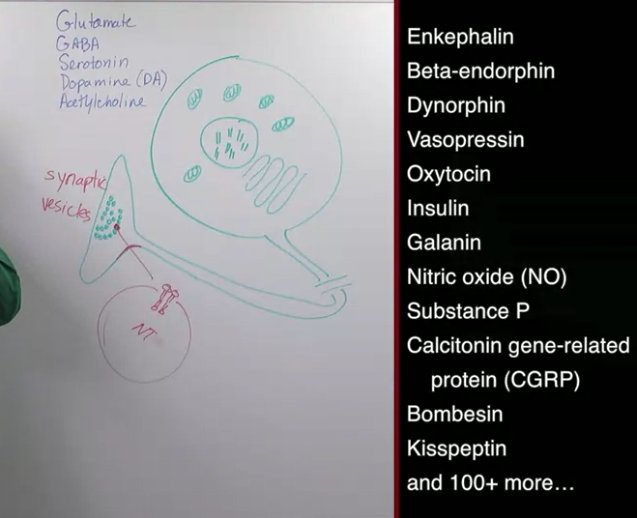
\includegraphics[width=10cm]{Neurtransmitters_SynapticVesicles.png}

}

Synthesis of neurotransmitters can be used as a theraputic tool. For instance,
in Parkinson's Disease, Dopamine isn't present, because the cells that make dopamine died.
\textbf{Mass Effect}: which means taking the starting chemical, the \textbf{substrate},
and through a series of enzymatic processes, create a synthesise a neurotransmitter,
and in the case of Parkinson's, Dopamine. Hence the substrace is used as the theraputic; examples are
Parcopa, Sinemet, etc.

\subsection{Neurotransmitter Release}
\paragraph*{}
How the neurotransmitters packaged in the synaptic vesicles to create a synapse.


\end{document}